\subsection{Motivation}
Deploying multi-agent systems in unstructured environments represents a critical frontier for modern autonomous systems beyond structured workspaces~\cite{yoshitake2019new, krnjaic2024scalable}.
Unlike controlled settings that benefit from reliable communication infrastructure, field deployments are fundamentally limited by intermittent networks and bounded energy reserves~\cite{mathew2015multirobot, calvo2025heterogeneous}.
When agents cross paths in these shared environments, their coupled motions require a decentralized right-of-way decision to determine which agent should proceed and which should yield~\cite{thomas2019right, celi2019deconfliction}.
In conventional approaches, resolving these spatial conflicts and preventing deadlocks requires bandwidth-intensive exchanges of complex planned trajectories or future task intents~\cite{wu2025decentralized, grover2023before}.
To drastically minimize this communication overhead, we propose energy-guided priority as a highly scalable coordination strategy. 
By exchanging only the energy sufficiency margin that predicts the energy remaining after task completion, agents can establish a unique, pairwise yielding order without relying on heavy trajectory sharing~\cite{notomista2018persistification, notomista2020persistification}.
This metric naturally scales to field constraints like sparse charging and complex missions, serving as a robust yielding cue for lifelong autonomy.

While this energy-guided priority is communication-efficient, its practical application must account for battery dynamics over long-term operations.
In practice, heterogeneous usage profiles naturally cause cell-specific battery degradation, introducing uncertainty even among identical hardware specifications. 
Rather than treating this uncertainty as a critical failure point, we seek to explicitly calibrate it to maintain a consistent and reliable precedence cue.

In this work, we estimate future energy requirements via a cell-specific proxy model and bound the residual prediction errors using adaptive conformal inference~\cite{gibbs2021adaptive}.
The resulting calibrated margins determine the discrete yielding order.
We then embed this precedence into a responsibility-aware control barrier function (CBF) formulation~\cite{cosner2023learning}.
Fig.~\ref{fig:main-figure} illustrates the overall idea: calibrated energy margins establish the yielding order, which is subsequently reflected in collision-avoidance responsibility.

\begin{figure*}[h!]
\centering
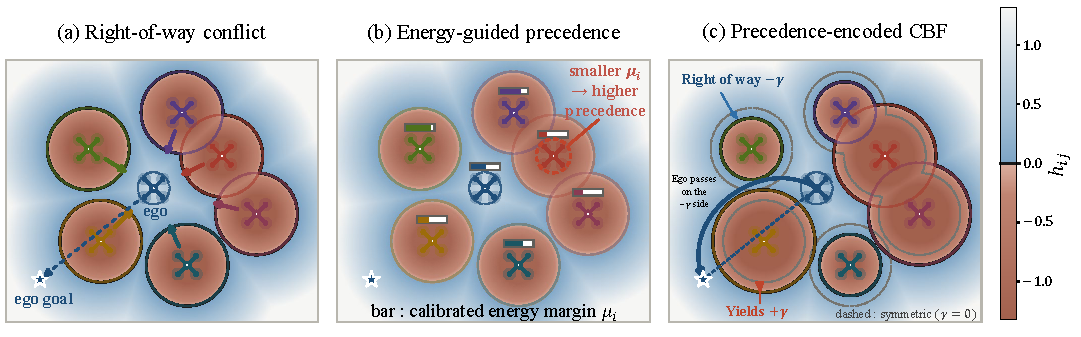
\includegraphics[width=\textwidth]{Figures/fig1_poc.pdf}
\caption{Energy-guided right-of-way coordination. (a) Multiple robots compete for right of way in a congested encounter. (b) Calibrated precedence cues $\mu_i$ determine a unique yielding order, where smaller $\mu_i$ indicates higher precedence and larger $\mu_i$ indicates greater flexibility to yield. (c) The order is encoded through a responsibility-aware CBF term ($\gamma$), assigning greater avoidance responsibility to the yielding robot while preserving pairwise safety.
\vspace{-10pt}
}
\label{fig:main-figure}
\end{figure*}

\subsection{Summary of Contributions}

We develop an uncertainty-calibrated energy-guided precedence rule for multi-robot right-of-way coordination and implement it using a responsibility-aware CBF formulation. 
Our main contributions are summarized as follows.

\textbf{Energy Sufficiency as a Precedence Criterion.} 
We use the energy expected to remain after task completion and travel to a charging station to determine pairwise right-of-way.
By exchanging only this scalar, agents establish a unique yielding order based on energy conditions, reducing communication overhead for conflict resolution.

\textbf{Uncertainty-Calibrated Energy Estimates.} 
We estimate the energy required to reach a charging station directly and after completing the assigned task using a battery-specific proxy model.
Adaptive conformal inference converts these predictions into bounds whose long-run violation rate is controlled at a prescribed level.
The resulting bounds define conservative precedence margins and an energy-sufficiency certificate with a conditional station-reachability guarantee.

\textbf{Safety-Preserving Precedence Integration.} 
We encode the precedence in a responsibility-aware CBF formulation by assigning unequal avoidance contributions within each interacting pair.
The paired local constraints preserve the underlying collision-avoidance condition regardless of which robot yields.
When multiple local right-of-way conflicts arise, all pairwise decisions follow a common energy-based ordering, thereby preventing cyclic precedence.


\subsection{Limitations and Future Works}
Our evaluations validate the efficacy of the energy-guided precedence cue within localized multi-agent encounters. 
However, confining this calibrated margin exclusively to a CBF formulation is inherently myopic for system-wide energy optimization. 
To achieve lifelong energy autonomy in disaster scenarios, future work will integrate this framework into higher-level mission planning architectures, such as global task allocation and long-horizon pathfinding.